\appendix
% \section{Statements}

% \subsection{Ethics Statement}
% This work adheres to the ICLR Code of Ethics. Our research is based on publicly available datasets (e.g., ImageNet-1K, ADE20K, Cityscapes, Pascal VOC) and does not involve human subjects, private data, or personally identifiable information. We follow standard licensing terms for all datasets used. The proposed framework, STELLAR, is a general-purpose method for self-supervised representation learning and is not designed for harmful or sensitive applications. 

% \subsection{Reproducibility Statement}
% We have made significant efforts to ensure the reproducibility of our results. Detailed descriptions of the STELLAR framework, training objectives, and experimental setups are provided in the main text and appendix. We report all datasets used, including preprocessing steps and evaluation protocols, and we describe ablation studies to clarify the contribution of each component. We will release the source code and pretrained model checkpoints after the internal review process to further facilitate reproducibility.

% \subsection{Use of Large Language Models}
% Large language models (ChatGPT) were used exclusively for language refinement, including polishing grammar, phrasing, and clarity of the manuscript. They were not used for research ideation, methodological design, experimental implementation, data analysis, or drawing conclusions. All scientific contributions of this work are entirely by the authors.


\section{Implementation Details}
\subsection{STELLAR Training}
We trained STELLAR with ViT models at size base, large, and huge, along with the latent queries, projection layers, clustering head, and a 6-layer ViT decoder. In the default setting, we initialized the ViT part in the encoder from public MAE checkpoint, and trained for 150 epochs for STELLAR-B, 100 epochs for STELLAR-L, and 50 epochs for STELLAR-H. We used 16 NVIDIA A100-80GB with batch size 128 each, totaling 2048. We used AdamW\citep{loshchilov2017decoupled} with base learning rate $1.5\times10^{-4}$ for STELLAR-B, and $5\times10^{-5}$ for STELLAR-L and STELLAR-H.

For concept clustering, we used 16384 prototypes for sparse and CLS tokens each. The projector is a 2-layer MLP before the prototype layer. We used 3 steps of Sinkhon-Knopp algorithm. The temperature in sparse-dense cosine similarity softmax is 0.06. We used 6-8 random masked views to align the sparse tokens, and additional 6-8 local crops to align the CLS token. Global views are of random scale 36\% to 100\%, and local view are of random scale 6\% to 36\%. We also apply color jittering, grascaling and Gaussian blurring.

In the ablation study of random prior, we trained the model from scratch and used exponential moving average (EMA) updated momentum encoder to encode the target prototype assignments in the warm-up stage. We EMA updated the full encoder (ViT, latent queries, projection, clustering head with momentum 0.996. The momentum encoder was used to encode a global view of the image into target prototype assignments, for both clustering loss and alignment loss. The masking ratio was 0.6 in the warm-up stage, and 0.8 during standard training. We trained the model with 150 epochs of EMA warm-up and 75 epochs of standard training.

\subsection{Evaluation Protocol}\label{eval}
For STELLAR and all baseline models, we evaluated the frozen feature from the pretrained model with linear probing. We used layer norm in classification tasks, and batch norm in segmentation tasks, followed by a single linear layer predicting the class of the image or patch. For all benchmarks, we split 10\% from the training set for validation. We tuned hyper-parameter with learning rate $1\times 10^{-5}, 2\times 10^{-5}, 5\times 10^{-5}, 1\times 10^{-4}, 2\times 10^{-4}, 5\times 10^{-4}, 1\times 10^{-3}, 2\times 10^{-3}, 5\times 10^{-3}, 1\times 10^{-2}$, and batch size 64, 128, 256, 512, 1024, 2048, 4096, 8192.

As the SSL methods varies across different baseline models, for classification tasks we used the mean-pooled feature from the representations where the corresponding SSL method was performed, e.g. the global CLS token for DINO, and dense patch tokens for MAE. We noticed the linear probing accuracy can vary depending on the pooling choice, and conducted experiments by using different types of tokens for each model, with results in Table \ref{pooling-table}. We observed that the SSL-ed are typically the best choice for linear probing, except for iBOT, which highly relies on the global CLS token for classification, even though the model was trained with MIM. In contrast, STELLAR and MAE are relatively more robust to token choices.


\begin{table}[hb]
\caption{ImageNet-1K linear probing accuracy (\%) by pooling different tokens. We mark in \textbf{bold} the tokens on which the specific SSL method was applied, and the top accuracy for each method.}
\label{pooling-table}
\begin{center}
\begin{tabular}{c|cc|cc|ccc|cc}
\multicolumn{1}{c}{}   & \multicolumn{2}{c}{DINO} &  \multicolumn{2}{c}{MAE} & \multicolumn{3}{c}{iBOT} &\multicolumn{2}{c}{STELLAR (ours)} \\
\hline 
tokens &  \textbf{global} & dense & global & \textbf{dense} & global & dense & \textbf{gl.+de.} & \textbf{sparse} &  dense \\
\hline 
lin. acc.  & \textbf{76.46} & 70.31 & 65.61 & \textbf{66.32} & \textbf{76.40} & 71.44 &  71.58 & \textbf{73.26} &  72.21
\end{tabular}
\end{center}
\end{table}

\begin{table}[hb]
\caption{List of baseline models and SSL method type.}
\label{tab:baselines}
\begin{center}
\begin{tabular}{l l c c c }
\multicolumn{1}{c}{\bf Model} &
\multicolumn{1}{c}{Reference} &
\multicolumn{1}{c}{Method} &
\multicolumn{1}{c}{SSL space} &
\multicolumn{1}{c}{SSL tokens}
\\ \hline 
BYOL & \cite{grill2020bootstrap} & augmentation alignment  &  latent & global \\
MoCo v3 & \cite{chen2021empirical} & contrastive learning  &  latent & global  \\
DINO & \cite{caron2021emerging} & augmentation alignment   &  latent & global \\
MSN  & \cite{assran2022masked}  & masked alignment  &  latent & global  \\
DenseCL & \cite{wang2021dense} & contrastive learning &  latent & dense \\
Data2Vec & \cite{baevski2022data2vec}  & latent MIM   & latent  & dense \\
SiameseIM & \cite{tao2023siamese}  &  latent MIM  & latent  & dense   \\
IJEPA & \cite{assran2023self}  &  latent MIM & latent  & dense   \\
iBOT & \cite{zhou2021ibot}  &  align + latent MIM  & latent  & global+dense  \\
BEIT & \cite{bao2021beit}  & token MIM  &  image  & dense \\
SimMIM  & \cite{xie2022simmim} & pixel MIM  & image  & dense  \\
MAE  & \cite{he2022masked}  & pixel MIM  &  image  & dense  \\
SemMAE  & \cite{li2022semmae}  & pixel MIM  &  image  & dense \\
TiTok  & \cite{yu2024image}  & reconstruction + clustering  &  image  & sparse  \\
AIM      & \cite{el2024scalable}  & autoregressive  & image & dense \\
DINOv2      & \cite{oquab2023dinov2}  & align + latent MIM   & latent & global+dense
\end{tabular}
\end{center}
\end{table}


\section{Additional Results}\label{app:results}


\subsection{Effect of pretraining data} 
We pretrained separate STELLAR versions on ImageNet-1K, Places365~\citep{zhou2017places} and compared their linear probing performance in Table \ref{data-table}.
\begin{table}[ht]
\caption{Effect of pretraining data.}
\label{data-table}
\begin{center}
\begin{tabular}{c|cc}
& \multicolumn{2}{c}{linear probing acc.} \\
 Pretraining data & ImageNet-1K & Places 365 \\
\hline 
ImageNet-1K & 76.94 & 49.25 \\
Places365 & 66.08 & 51.98
\end{tabular}
\end{center}
\end{table}

\subsection{Semantics from different features} 
We conducted linear probing of different mean-pooled features of different types, and compared in Table \ref{feat-table}. Sparse feature showed strongest global understanding quality.
\begin{table}[ht]
\caption{Semantics in different features}
\label{feat-table}
\begin{center}
\begin{tabular}{c|ccc}
 Feature & sparse & cls & dense \\
\hline 
IN-1K lin. acc (\%) & 73.26 & 72.23 & 72.21 
\end{tabular}
\end{center}
\end{table}


\subsection{Concept alignment with language}
Inspired by \cite{zhang2025assessing}, we used frozen feature from STELLAR and aligned with the text tower of CLIP~\citep{radford2021learning} with a single attention pooled probing layer. The evaluation on vision language tasks with comparison to baseline models are shown in Table \ref{vlm-table}.

\begin{table}[ht]
\caption{Language alignment evaluation.}
\label{vlm-table}
\begin{center}
\begin{tabular}{c|cc|cc|cc|c}
\multicolumn{1}{c}{}   & \multicolumn{2}{c}{IN-1K 0-shot} &  \multicolumn{2}{c}{MS COCO} & \multicolumn{2}{c}{Winoground} & MMVP \\
\hline 
  &      @1  & @5 & T2I & I2T & Text & Image & Avg. \\
\hline 
MAE &   23.18 & 50.43 & 11.28 & 13.46 & 20.75 & 9.00 & 19.26 \\
iBOT &  50.01 & 80.43 & 20.79 & 29.38 & 24.75 & 12.00 & 18.52 \\
STELLAR &   51.53 & 80.04 & 17.94 & 22.34 & 26.25 & 8.25 & 19.26 \\
\hline
CLIP  &  72.7 & - & 43.0 & 59.7 & 30.5 & 11.5 & 20.0
\end{tabular}
\end{center}
\end{table}

\subsection{Finetuning}
We performed finetuning for STELLAR on ImageNet-1K classification and ADE20K segmentation, and compared with baseline models. We used the same evaluation protocol as in Sec. \ref{eval}, with the backbone unfrozen and finetuned for 75 epochs. We used ViT-B for all models. The finetuning results are shown in Table \ref{finetune-table}. STELLAR showed consistent performance gain across different tasks, and close to the top model iBOT with slight difference.


\begin{table}[ht]

\caption{Finetuning performance in ImageNet-1K classification accuracy and ADE20K segmentation mIOU (\%). We show in parentheses the gain over the respective linear probing results.}
\label{finetune-table}
\begin{center}
\begin{tabular}{c|ccc}
 Model & ImageNet-1K Acc. & ADE20K mIOU \\
\hline 
DINO & 79.58 (+3.12) & 39.22 (+12.35) \\
MAE & 77.75 (+11.43) & 40.33 (+9.42) \\
iBOT & 80.72 (+9.14) & 42.76 (+10.97) \\
\hline
STELLAR & 80.05 (+6.78) & 41.98 (+10.65)
\end{tabular}
\end{center}
\end{table}


\subsection{Efficiency analysis}
To analyze the efficiency of the STELLAR framework, we printed the processing time of the main components in the STELLAR framework with one A100 GPU at different batch sizes. Encoding the main global view of the image takes up most of the processing time, followed by encoding the masked views (8 views at 80\% masking ratio) and decoding to the original image. The Sinkhorn-Knopp algorithm used for clustering and the Sinkhorn algorithm used in optimal transport matching take up much less amount of time, and their total processing time stay at similar level when increasing the batch size. 

In comparison to the Sinkhorn matching algorithm we used in our experiments, we show the processing time using an alternative Hungarian matching algorithm commonly used in previous literature such as Sparse R-CNN~\citep{sun2021sparse}, DETR~\citep{carion2020end} and MaskFormer~\citep{cheng2021per}. As the implementation of the exact matching is not scalable with GPU parallelization, it's computational time increases linearly with the batch size. At batch size 64, it is already 6 times of the encoder processing, while the Sinkhorn algorithm is over 100 times faster. For this reason, we added a small entropy regularization term in the bipartite matching objective, allowing us to use the Sinkhorn algorithm for efficient matching with GPU parallelization.

\begin{table}[ht]
\caption{Processing time (s) of the main components in the STELLAR framework with one A100 GPU at different batch sizes. In comparison to the Sinkhorn matching algorithm we used in our experiments, we show the processing time using an alternative Hungarian matching algorithm commonly used in previous literature (shown in gray).}
\label{finetune-table}
\begin{center}
\begin{tabular}{c|ccccc}
 Batch size & 4 & 8 & 16 & 32 & 64  \\
\hline 
Encoder & 8.2 $\times 10^{-3}$ & 9.1 $\times 10^{-3}$ & 1.4 $\times 10^{-2}$ & 2.0 $\times 10^{-2}$ & 3.2 $\times 10^{-2}$ \\
Decoder & $4.6 \times 10^{-3}$ & 6.8 $\times 10^{-3}$ & 8.8 $\times 10^{-3}$ & 1.2 $\times 10^{-2}$ & 1.5 $\times 10^{-2}$ \\
Mask encoding & $7.9 \times 10^{-3}$ & 8.9 $\times 10^{-3}$ & 1.1 $\times 10^{-2}$ & 1.8 $\times 10^{-2}$ & 1.7 $\times 10^{-2}$\\
SK clustering & $3.4 \times 10^{-4}$ & 3.4 $\times 10^{-4}$ & 3.4 $\times 10^{-4}$ & $3.7 \times 10^{-4}$ & 3.9 $\times 10^{-4}$  \\
Sinkhorn matching & $1.4 \times 10^{-3}$ & 1.4 $\times 10^{-3}$ & 1.4 $\times 10^{-3}$ & $1.4 \times 10^{-3}$ & 1.2 $\times 10^{-3}$ \\
\hline
\color{gray}{Hungarian matching} & \color{gray}{$5.7 \times 10^{-3}$} & \color{gray}{1.7 $\times 10^{-2}$} & \color{gray}{4.0 $\times 10^{-2}$} & \color{gray}{9.0 $\times 10^{-2}$} & \color{gray}{1.8 $\times 10^{-1}$}
\end{tabular}
\end{center}
\end{table}


% \begin{table}[t]
% \caption{Model performance with different configurations}
% \label{mse-table}
% \begin{center}
% \begin{tabular}{cccccc|cc}
% \# tk.  & \multicolumn{1}{c}{Recon.}  &\multicolumn{1}{c}{Cluster} &  Set align & CLS align & KoLeo & IN1k lin. & ADE lin. \\
% \hline \\
% 8 &    code  & \checkmark & \checkmark & \checkmark & \checkmark & 72.97 & 31.04 \\
% 16  &   code    & \checkmark  & \checkmark & \checkmark & \checkmark & 73.26 & 31.33\\
% \hline 
% \multicolumn{8}{l}{\it Ablation models versions} \\
% 8 &    pixel  & \checkmark & \checkmark & \checkmark & \checkmark & 72.16 (-0.81) & 30.04 (-1.00) \\
% 16  &  \ding{55}   & \checkmark  & \checkmark & \checkmark & \checkmark & 72.44 (-0.82) & 29.94 (-1.39) \\
% 16  &   code    &  \ding{55}   &  \ding{55}  &  \ding{55}  & \checkmark & 52.07 (-21.19) & 20.46 (-10.87) \\
% 16  &   code    & \checkmark  & \ding{55}  & \ding{55}  & \checkmark & 2.73 (-70.53) & 1.93 (-29.39) \\
% 16  &   code    & \checkmark  & \checkmark & \ding{55}  & \checkmark & 70.79 (-2.47) & 30.20 (-1.12) \\
% 16  &   code    & \checkmark  & \checkmark & \checkmark & \ding{55}  & 72.05 (-1.21) & 30.10 (-1.23) \\
% \end{tabular}
% \end{center}
% \end{table}




\section{Additional Illustration}
See Fig.~\ref{fig:stellar} and \ref{fig:align}.
\begin{figure}
    \centering
    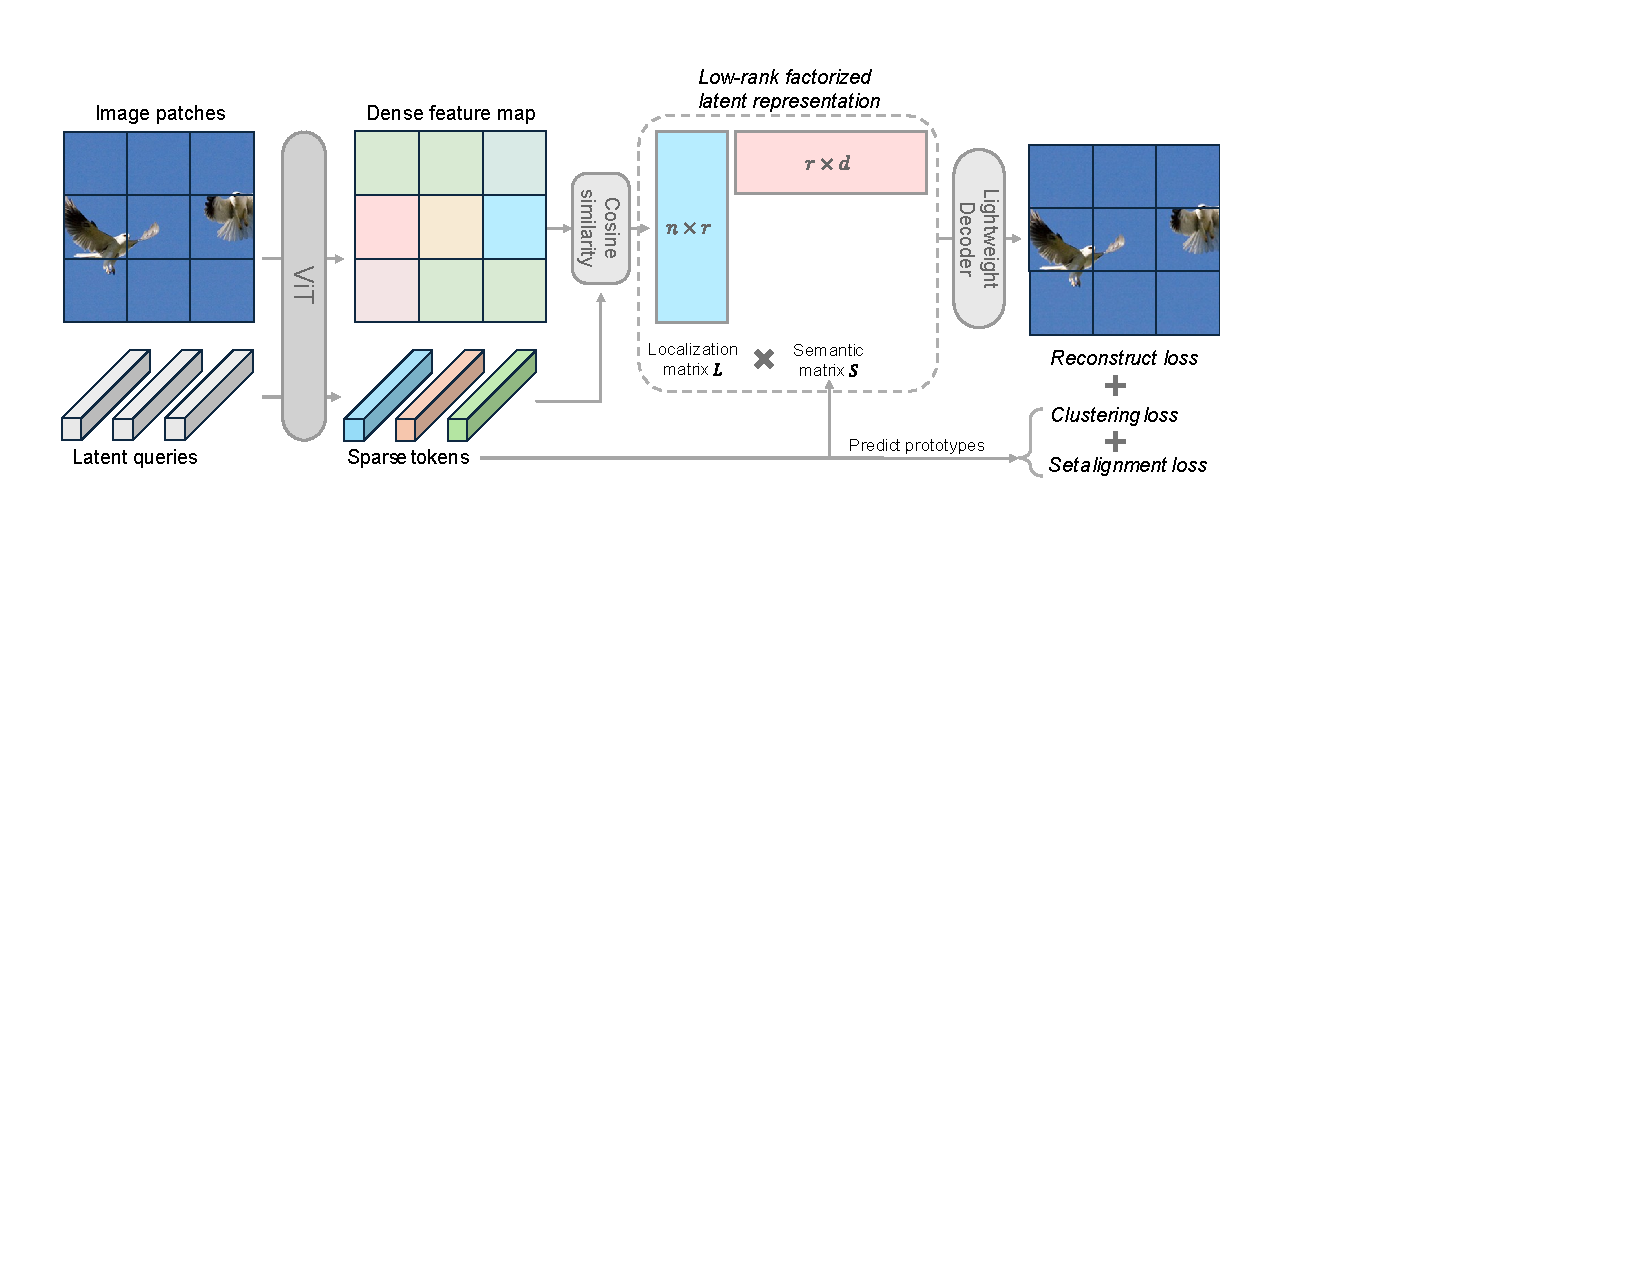
\includegraphics[trim={1cm 13.5cm 7cm 1cm},clip, width=\linewidth]{figures/stellar.pdf}
    \caption{\small The STELLAR framework. We use a vanilla ViT to extract sparse tokens from an image, and model the latent representation as a low-rank matrix factorization, ensuring reconstruction of the original image. Clustering loss and set alignment loss are applied on the disentangled sparse tokens.}
    \label{fig:stellar}
\end{figure}
\begin{figure}
    \centering
    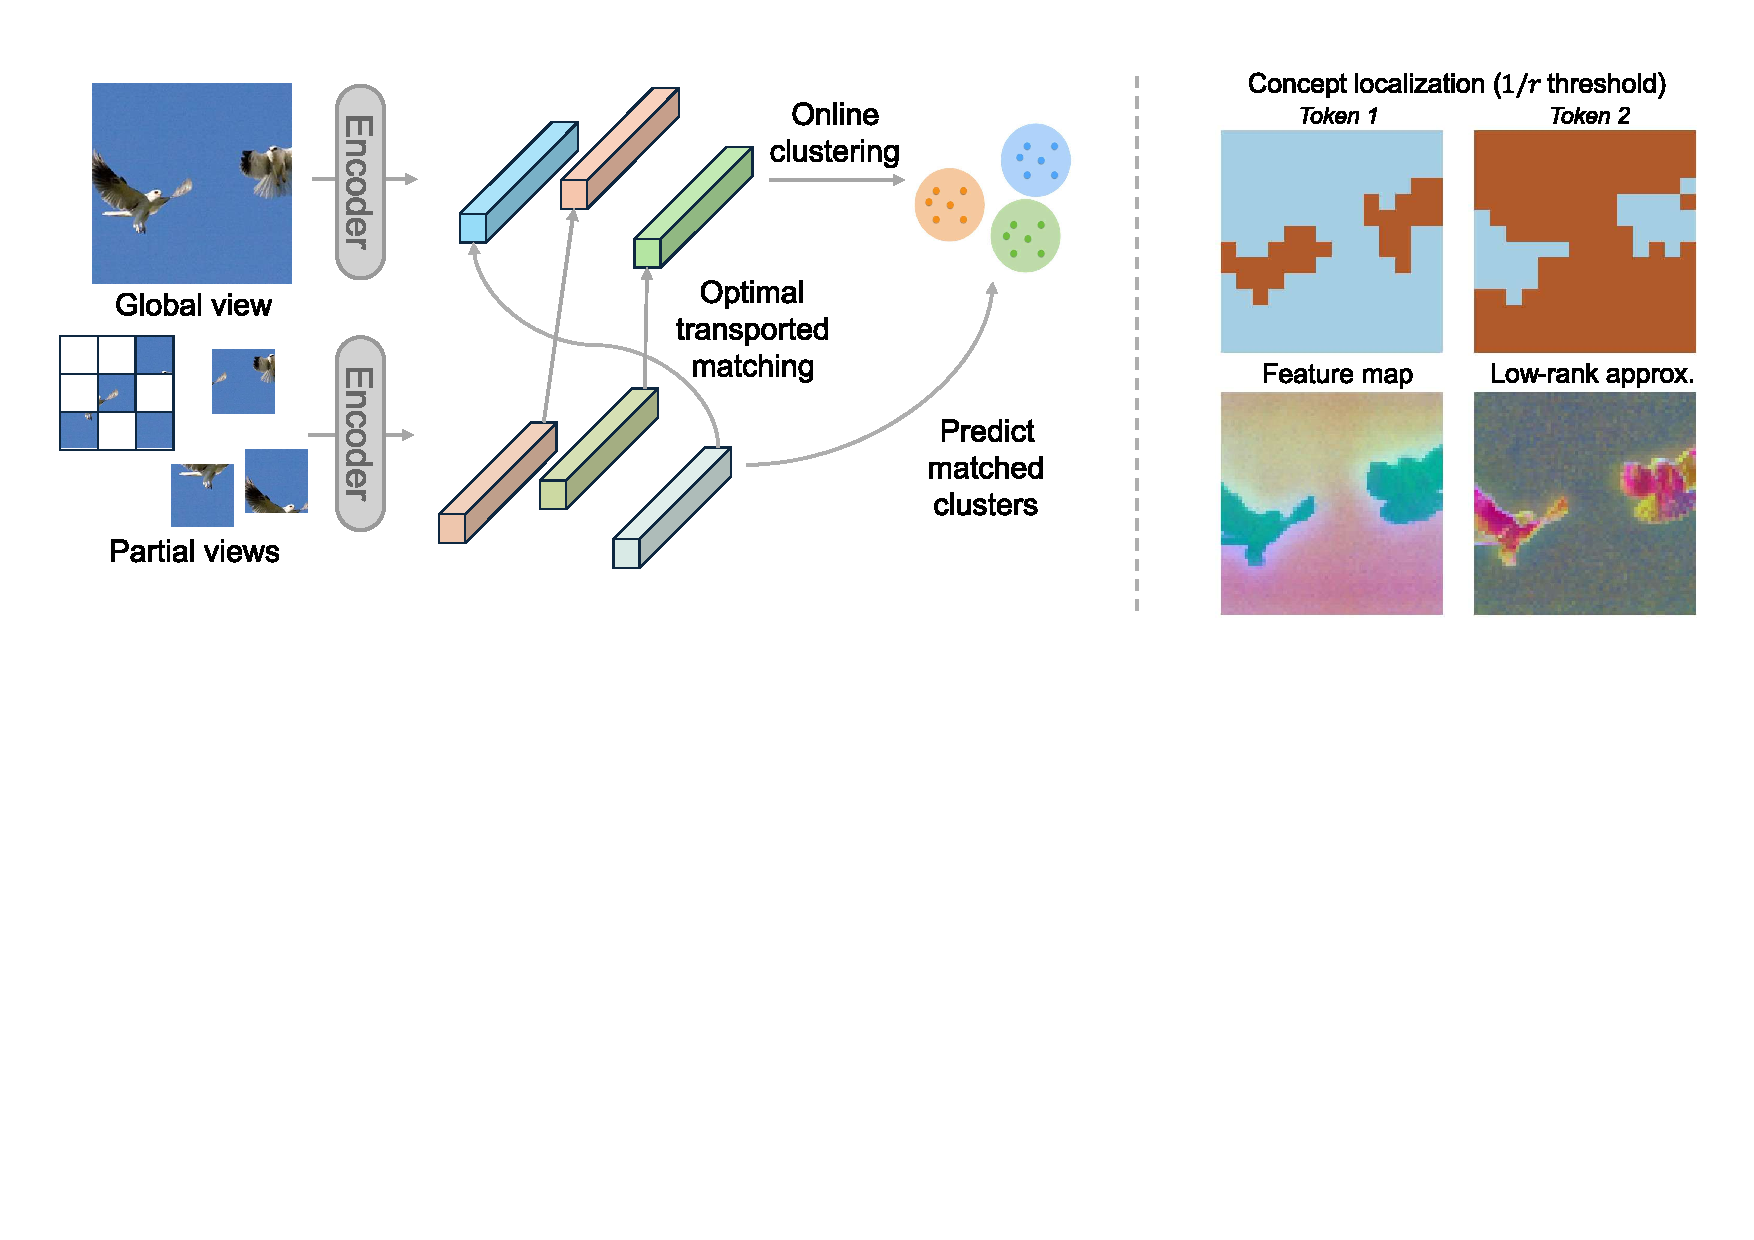
\includegraphics[trim={1cm 10.5cm 1cm 1cm},clip, width=\linewidth]{figures/match-viz.pdf}
    \caption{\small Left: Concept clustering and alignment workflow. Right: visualization of learned representation.}
    \label{fig:align}
\end{figure}